
\item A bi-convex lens is formed with two thin plano-convex lenses as shown in the figure. Refractive index \( n \) of the first lens is 1.5 and that of the second lens is 1.2. Both the curved surfaces are of the same radius of curvature \( R = 14 \) cm. For this bi-convex lens, for an object distance of 40 cm, the image distance will be
    \begin{center}
        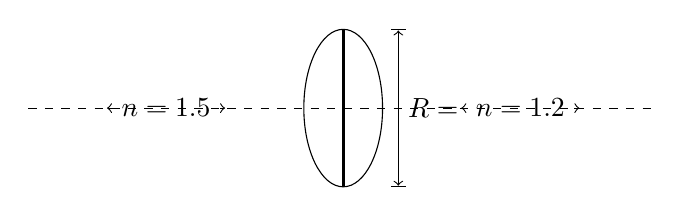
\begin{tikzpicture}
            \draw[very thick] (0,0) -- (0,2);
            \draw (0,1) ellipse (0.5 and 1);
            
            \draw[|<->|] (0.7,0) -- node[right] {\( R=14 \) cm} (0.7,2);
            \draw[<->] (-3,1) -- node[fill=white] {\( n=1.5 \)} (-1.5,1);
            \draw[<->] (1.5,1) -- node[fill=white] {\( n=1.2 \)} (3,1);
            
            \draw[dashed] (-4,1) -- (4,1);
        \end{tikzpicture}
    \end{center}
    \begin{tasks}(2)
        \task \( -280.0 \) cm.
        \task \( 40.0 \) cm.
        \task \( 21.5 \) cm.
        \task \( 13.3 \) cm.
    \end{tasks}
